\documentclass{article}
\usepackage[utf8]{inputenc}
\usepackage{amsmath}
\usepackage{url}
\usepackage[margin=0.75in]{geometry}
\usepackage{graphicx}
\usepackage[export]{adjustbox}
\usepackage{float}
\setlength{\parskip}{0.7em}
\setlength{\parindent}{0em}

\begin{document}
	\begin{center}
		
		% MAKE SURE YOU TAKE OUT THE SQUARE BRACKETS
		\LARGE{\textbf{CSE 6730,Final Report}} \\
		\vspace{1em}
		\Large{Project 2: Complex Simulation} \\
		
	\end{center}
	\begin{normalsize}
		
		\section{Project Title}
		
		Simulation of Predator-Prey Population Dynamics 
		
		\section{Team Members}
		
		\begin{enumerate}
			\item D. Aaron Hillegass (GTID 901988533)
			\item Siawpeng Er (GTID 903413430)
			\item Xiaotong Mu (GTID 903529807)
		\end{enumerate}
	
		\section{Github}
		Currently, the github is at https://github.gatech.edu/ser8/complex-sys.
		The final submission for checkpoint and final project will be at the Folder Submission with each subfolder.\\

		For the ABS model, we create one model with interaction but it is conflicting with macbook pro touch bar for one of our member laptop and the laptop shut down every time the code was executed. Running on other member laptops is completely fine. \\
		We create one embedded version prior the GUI version as well. Embedded version suppor the step through function that allow user to look at each step.

		
		\section{Problem Description and Purpose}
		The predator and prey relationship is an important ecological system. Their populations rise and fall over time as they interact and impact one another. These interactions are the prime movers of energy through food chains. Both prey and predators are affecting each other. \cite{laham_2012_a}In simplest interaction, predators depend on the prey as the food source. However, any abuse of the food source may result in decease in population of the prey, and subsequently decrease the number of the predators due to lack of food. Because of such interaction, the population of the predators and the prey may oscillate, and inversely proportional to each others.\cite{obaid_2013_the}\
		
		The predator-prey relationship is important for us to understand the impact of the relationship on the ecological system in one area. Such relationships are always complicated. Without predators, prey (normally herbivores) will cause detrimental impact on the plants in that area. However, overkill by the predators may also impact the balance of the nature. Besides, there are effects from human intervention on such relationship (eg: hunting and destroy of the habitat). Furthermore, predator-prey model can be used to describe many fundamental characteristics of ecological systems and can even be extended to other ideas like military response \cite{derrik}.\\
		
		One of the mathematical models that simulates predator-prey interactions is the Lotka-Volterra model proposed by Alfred Lotka and Vito Volterra. Lotka helped develop the logistic equation to explain auto-catalytic chemical reactions. Volterra interconnected the logistic equation to two separate populations in competition to explain predator and prey relationships. We hope to use this intuitive model in our complex system simulation, so that we could gain understanding of these relationships, as well as the impact of our activities on them. Furthermore, we would like to investigate the equilibria and stability of our ecological system, and to facilitate in understanding the general behavior of the system by finding the equilibrium solutions of a coupled set of nonlinear ordinary differential equations.\cite{tung_2007_topics}\cite{a2018_alfred}
		\section{General Assumptions}
		Important refinements such as environmental heterogeneities, more complex food web networks, and different functional responses will be selectively added to future models in iterative process. The following assumptions are made with current model:
		\begin{itemize}
		    \item The environment is assumed homogeneous with no natural disasters or  variations in temperature
		    \item All species are of the same size, produce the same amount of resources when consume%, and share the same set of simple strategic rules
		    \item No limited lifetime for preys and predators
		    \item Each prey or predator has a fixed probability of reproducing at each time step.
		    \item Unlimited food available to the prey is assumes, and so the prey(and predator)growth rates are limited by corresponding capacity and growth coefficients
		    \item Each predator eats a constant proportion of the prey population per year; In other words, doubling the prey population will double the number eaten per predator, regardless of how big the prey population is.
		    \item Predator reproduction is directly proportional to prey consumed; another way of expressing this is that a certain number of prey consumed results in one new predator; or that one prey consumed produces some fraction of a new predator.
		    \item A constant proportion of the predator population dies per year. In other words, the predator death rate is independent of the amount of food available.
		\end{itemize}

		\section{Literature Review}
		Simple predator and prey interaction could be model using Lotka-Volterra model. In our model, we borrow idea from \cite{Sayama2013} to build firstly our simple interaction model. Firstly, our rabbit model is following the  
		\begin{equation}
		R_t = R_{t-1} + growth_{R} \times \big( \frac{capacity_{R} - R_{t-1}}{capacity_{R}} \big) R_{t-1}
		\end{equation}
		For the coyote,
		\begin{equation}
		\begin{aligned}
		C_t  & \sim (1 - death_{C}) \times C_{t-1} \\
		&= C_{t-1} - death_{C} \times C_{t-1}
		\end{aligned}
		\end{equation}
		
		With the simple interaction from the first two parts, now we can combine both interaction and come out with simple interaction between the two species.
		\begin{equation}
		R_t = R_{t-1} + growth_{R} \times \big( \frac{capacity_{R} - R_{t-1}}{capacity_{R}} \big) R_{t-1} - death_{R}(C_{t-1})\times R_{t-1}
		\end{equation}
		
		\begin{equation}
		C_t = C_{t-1} - death_{C} \times C_{t-1} + growth_{C}(R_{t-1}) \times C_{t-1}
		\end{equation}
		
		In equations above, death rate of rabbit is a function parameterized by the amount of coyote. Similarly, the growth rate of coyotes is a function parameterized by the amount of the rabbit. The death rate of the rabbit should be $0$ if there are no coyotes, while it should approach $1$ if there are many coyotes. One of the formula fulfilling this characteristics is hyperbolic function.
	
		\begin{equation}
		death_R(C) = 1 - \frac{1}{xC + 1}
		\end{equation}
	
		where $x$ determines how quickly $death_R$ increases as the number of coyotes ($C$) increases. Similarly, the growth rate of the coyotes should be $0$ if there are no rabbits, while it should approach infinity if there are many rabbits. One of the formula fulfilling this characteristics is a linear function.
	
		\begin{equation}
		growth_C(R) = yR
		\end{equation}
	
		
		where $y$ determines how quickly $growth_C$ increases as number of rabbit ($R$) increases.
		
		Putting all together, the final equtions are
		
		
		\begin{equation}
		R_t = R_{t-1} + growth_{R} \times \big( \frac{capacity_{R} - R_{t-1}}{capacity_{R}} \big) R_{t-1} - \big( 1 - \frac{1}{xC_{t-1} + 1} \big)\times R_{t-1}
		\end{equation}
		\begin{equation}
		C_t = C_{t-1} - death_{C} \times C_{t-1} + yR_{t-1}C_{t-1}
		\end{equation}
% 		To investigate the equilibria and stability of the system, we will be using the Lotka-Volterra set of equations with Holling's Type II functional response, the model can be described by
%         \begin{equation}	
% 		\frac{dx}{dt} = ax-bxy
% 		\frac{dy}{dt} = dbx \times y - cy
% 		\end{equation}
		
		The previous relationship could be extended to multiple predators and preys relationship. In the multiple predators and preys model, we will be focusing on a specific 2+2 model with two preys: rabbits and deers ,and two predators: coyotes and wolfs. We assume that each predator preys on each prey but not on each other. And the preys population capacity are affecting each other:
		\begin{equation}
		    capacity_{D} = capacity_{prey} - capacity_{R}
		\end{equation}
		What difference from the simple predator and prey interaction is that, now the death rate of preys is a function parameterized by both the amount of coyotes and the amount of wolfs. 
		\begin{equation}
		    death_R(C,W) = (1 - \frac{1}{xC + 1}) + (1 - \frac{1}{vW + 1})\\
		\end{equation}
		\begin{equation}
		    death_D(C,W) = (1 - \frac{1}{xC + 1}) + (1 - \frac{1}{vW + 1})\\
		\end{equation}
		
		where v determines how quickly $death_{R}$ increases as the number of wolfs (W) increases. 
		Similarly, the growth rate of predators is a function parameterized by the amount of both rabbits and deer.  Where u determines how quickly $growth_W$ increases as number of rabbit (R) increases, and $D_{t}$ represents the number of deer at time t.\\
		
		\begin{equation}
		growth_C(R) = yR+uD
		\end{equation}
		\begin{equation}
		growth_W(R) = yR+uD
		\end{equation}
		
		Multiple Prey Multiple Predator model is described in the following equations:
		
		\begin{equation}
		R_t = R_{t-1} + growth_{R} \times (\frac{capacity_R - R_{t-1}}{capacity_R})R_{t-1} - (1 - \frac{1}{xC_{t-1} + 1} ) \times R_{t-1}- (1 - \frac{1}{vW_{t-1} + 1})\times R_{t-1}
		\end{equation}
		\begin{equation}
		D_t = D_{t-1} + growth_{D} \times (\frac{capacity_D - D_{t-1}}{capacity_D})D_{t-1} - (1 - \frac{1}{xC_{t-1} + 1} )\times D_{t-1}- (1 - \frac{1}{vW_{t-1} + 1})\times D_{t-1}
		\end{equation}

		
		
		\begin{equation}
		    C_{t} = C_{t-1} - death_C \times C_{t-1} + yR_{t-1}C_{t-1} + u D_{t-1}C_{t-1}
		\end{equation}
		\begin{equation}
		    W_{t} = W_{t-1} - death_W \times W_{t-1} + yR_{t-1}W_{t-1} + u D_{t-1}W_{t-1}
		\end{equation}
		\section{Data Source}
		For this project, we do some simple simulation between rabbit and coyote. We obtained the idea from the Wikipedia for rabbits and coyotes growth and reduction rate.
	
		\section{Methodology}
		Our simulation will first simulate predators and prey entering and exiting a predefined area. Then through interactions, their population may affecting each others.
		
		Traditionally, there is the nonlinear Lotka-Volterra Model of the predator-prey dynamic system \cite{inproceedings, 1102729}. LVM approach is a simplified model and suitable for detailed stability analysis. However, it is also very limited model and lack of flexibility for complex interaction. Hence, we also hope to incorporate the Agent-Based Model \cite{Hodzic} in this project to increase the completeness of our analysis. We gained most of insight of writing our simulation based on \cite{Sayama2013}. We also include another way to do the simulation through cellular automata.
		
		In our project, some of the ideas that we wish to investigate include:
		\begin{enumerate}
			\item Long-term population interaction among predators and prey.
			\item Introduction of the uncertainties like diseases.
			\item Introduction of the third parties interaction: human activity, natural disasters etc.
		\end{enumerate}
		
		\section{Development Platform}
		The programming language is Python 3. We will provide a Jupyter notebook for user interaction.
		In the Jupyter notebook, we will allow the user to change some of the probability and the simulation parameters to see different result of the simulation.
		
		\subsection{Lotka-Volterra Model}
		The Lotka-Volterra Model is a classic model of predator-prey interactions. It is based on a pair of first order non-linear differential equations. Volterra first proposed simple model for the predation of one species by another to explain the oscillatory levels of a certain population. In the continuous time model, if x(t) is the prey population and y(t) is the predator population at time t, the Volterra's model is:
		$$\frac{dx}{dt} = ax-bxy$$
		$$\frac{dy}{dt} = cxy - dy$$
		where a, b, c and d are all positive constants.\\
		The exponential growth for prey is represented by the term ax, and the prey population is simultaneously destroyed by predators, and the rate of predation upon the prey is assumed to be proportional to the rate at which the predators and prey meet,that is represented by bxy. Also, we can tell by looking at the equation $\frac{dx}{dt}$, if either x or y is equal to zero, then there is no predation. In $\frac{dy}{dt}$, the cxy is the prey's contribution to predators growth rate, and it is assumed to be proportional to the size of available prey as well as the population of predator, the xy can be thought of as the conversion of energy from the food source. -dy is the exponential decay in predator population due to lack of food. The equations above demonstrates a simple explanations of how prey and predator population fluctuate. 
		Furthermore, If the number of prey becomes sufficiently great, then the prey may be interfering with each other in their quest for food and space. One way to describe this effect mathematically is to assume that the prey not grows indefinitely in the absence of predators, but will ultimately reach the carrying capacity of the environment. Hence prey doesn't grow exponentially but follow a logistic growth equation as below:
		$$\frac{dx}{dt} = ax(1-\frac{x}{K})-bxy$$
		$$\frac{dy}{dt} = y(cx-d)$$
		where K is the saturation constant.\\
		By applying forward Euler method to the set of ODEs above, we obtain the discrete time Lotka-Volterra Model.
		$$x_{t} = x_{t-1}+ax_{t-1}(1-\frac{x_{t-1}}{K})-bx_{t-1}y_{t-1}$$
		$$y_{t} = y_{t-1}+y_{t-1}(cx_{t-1} - d)$$		
		In order to come up with mathematical form for b and c, we should consider the extreme cases.
		If there is no predator, the death rate for prey should be zero, and it should approach one as predator population keep increasing. With the equations above, we can determine the equilibrium points of the system, and then investigate their stability. Equilibrium points can be determined by setting $x_{t}$ and $y_{t}$ equal to $x_{t-1}$ and $y_{t-1}$ respectively, then solving the the nonlinear equations. After we determined the existence of the equilibrium points of the Lotka–Volterra models, we could further investigate their stability by calculating the eigenvalues for the Jacobian matrix of the Lotka– Volterra models at each equilibrium point of them. To better illustrate the patterns we can fix the parameters with some initial values and generate the phase portrait of the system. By looking at the plot [Fig 11] we can observe that every trajectory in the first quadrant is a closed curve. Thus the predator and prey populations oscillate go in cycles.
		
		Currently, we have successfully model the world, rabbits and coyotes. Since this is a step by step tutorial based project, we first create the simulation with only the rabbits growth rate, and coyotes death rate. Finally, we allow some interaction between rabbits and coyotes. This is the first phase of our Lotka-Volterra Model.
		
		In the program, simply run python notebook for the current main.ipynb. The tutorial should be self contained. Some of the current parameters that could be play with is as per table below
		
	\begin{center}
		\begin{tabular}{ |c|c|} 
			\hline
			Parameter & Description  \\ 
			\hline
			\multicolumn{2}{|c|}{Single Rabbit Model} \\
			\hline
			Initial population & Initial rabbit population \\ 
			Capacity & Capacity of the environment\\ 
			Growth rate & How fast rabbit could grow \\ 
			\hline
			\multicolumn{2}{|c|}{Single Coyote Model} \\
			\hline
			Initial population & Initial coyote population \\ 
			Death rate & How fast coyote could decrease \\ 
			\hline
			\multicolumn{2}{|c|}{Coyote Rabbit Interaction Model} \\
			\hline
			Initial rabbit population & Initial rabbit population  \\ 
			Capacity & Capacity of the environment\\ 
			Growth rate & How fast rabbit could grow \\ 
			Initial coyote population & Initial coyote population \\ 
			Death rate & How fast coyote could decrease \\ 
			x & How fast rabbit decrease due to the coyote population \\
			y & How fast coyote increase due to the rabbit population \\
			\hline
			\multicolumn{2}{|c|}{Multiple Preys and Predators Model} \\
			\hline
			Initial prey population & Initial rabbit and deer population \\ 
			Capacity & Capacity of the environment and capacity of rabbit\\ 
			Growth rate of each prey & How fast rabbit and deer could grow \\ 
			Initial predator population & Initial coyote and wolf population \\ 
			Death rate of each predator & How fast coyote and wolf could decrease \\ 
			Death rate ratio due to coyote & How fast rabbit and deer decrease due to the coyote population \\
			Death rate ratio due to wolf & How fast rabbit and deer decrease due to the wolf population \\			
			Growth rate ratio due to rabbit & How fast coyote and wolf increase due to the rabbit population\\
			Growth rate ratio due to deer & How fast coyote and wolf increase due to the deer population\\
			\hline
		\end{tabular}
	\end{center}

	\subsection{Cellular Automata}
		We have cellular Automata that include space constraint on the prey and predator relationship. The prey and predator is playing "hide and seek" where predator can only eat those within its neigbhorhood. We define the neighborhood as up, down, left and right location of the cell. That is, we follow the von Neumann neighborhoods.
		Cellular rules:
		
		\begin{center}
			\begin{tabular}{ |c|c|} 
				\hline
				Parameter & Description  \\ 
				\hline
				World size & The canvas size in nxn dimension  \\ 
				Maximum predator & How many predator initialized\\ 
				Prey reproductive probability & Probability of prey reproduce \\ 
				Predator reproductive probability & Probability of predator reproduce with prey around \\ 
				Predator dying probability & Probability of predator die if no prey around \\ 
				Maximum step  & maximum step run for the cellular automata \\ 
				\hline
			\end{tabular}
		\end{center}
	
		\subsection{Agent Based Simulation}
		In population dynamics we generally analyze either how a single population changes over time, or how two populations interact and influence their population sizes over time. The role of decision making by individual spiecies is largely ignored in the simulation models of ecology, such as Lotka-Volterra model we mentioned previously. To better understand how modeling helps link individual behaviors to phenomena at the level of population interaction, we want to  introduce agent based modeling.
		 Agent-based modeling brings understanding and clarity to complex natural interactions by allowing them to develop through the individuals. This individual development can provide added realism over other modeling approaches. In agent based model,
		agents can be born and die during a simulation, and certain rules are defined for encounters between individuals. This means that the number of state variables involved in a system can change dynamically over time.
		Agent rules:
		\begin{itemize}
		    \item For prey each individual agent reproduces at a certain reproduction rate
		    \item If a prey agent meets a predator agent, it dies with some probability because of predation
		    \item Predator agent  dies with certain probability if no prey nearby
		    \item Predators can diffuse a little faster than prey
		    \item To handle situations where the size of the agent population changes rapidly, we assume in each asynchronous updating,
$\frac{1}{agent\ population}$ of a unit length of time passes by
		\end{itemize}
		
		We improve our model to Agent Based Model for the same relationship. We have one gui interaction model, and another static model populate the outcome of interaction.
		
			\begin{center}
			\begin{tabular}{ |c|c|} 
				\hline
				Parameter & Description  \\ 
				\hline
				Initial rabbit count & Initial rabbit population  \\ 
				Rabbit capacity & Capacity of the environment\\ 
				Rabbitreproduction & How fast rabbit could grow \\ 
				Initial coyote count & Initial coyote population \\ 
				Coyote death rate & How fast coyote could decrease \\ 
				Coyote birth rate  & How fast coyote could increase \\ 
				\hline
			\end{tabular}
		\end{center}
		
		\subsection{Event-Based Simulation}
		
		We covered event-based simulations in the first half of the course. We modeled the predator-prey this way as well.  The result runs slowly and takes up a lot of memory, but it enables us to model some of the more subtle effects:
		\begin{itemize}
		\item the delay between birth and sexual maturity
		\item the effects of fluctuating nutrition during pregnancy
		\item the effects of over-grazing by herbivores
		\item the natural lifespans of the predator and the prey
		\end{itemize}
		
		In this model, each coyote and each rabbit are entities.  Grass is a resource that gradually renews.  Every mating and every resulting birth are events, governed by the gestation period and litter size of the animal.  When each animal is created, its natural death is added to the queue. (Few rabbits ever made it to their natural death, however.)
	
		\section{Tutorial}
		The tutorial is divided into two portion. One is the basic Lotka-Volterra Model. Another is the Agent Based Simulation Model. Both the tutorials are run on Jupyter Notebook.
		\subsection{Lotka-Volterra Model}
		\subsubsection{Introduction}
		Project topic: \textbf{Simulation of Predator-Prey Population Dynamics }\\
		our model is single relationship, multiple relationship Our prey are rabbits and deers, while the predators are coyote and wolves.
		Pending for screenshot
		\subsubsection{Part 1: Rabbits without predators}
		In part 1 of the tutorial, first we introduce a relationship for a prey (rabbits) without predators. The default capcity of 605 is chosen by making some assumption. Here, we introduce the formula used. 
			\begin{figure}[H]
			\frame{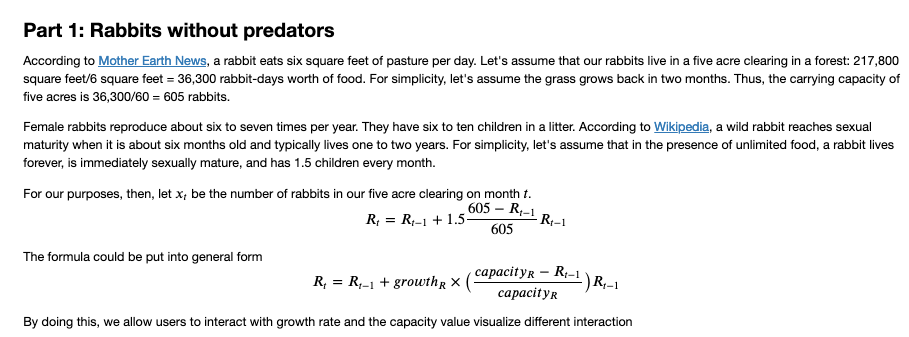
\includegraphics[width = \linewidth, frame]{Figures/0}}
			\caption{Introduce rabbit population without predators formula}
			\end{figure}
		
		Then, we allow users to change the default value of initial rabbit population,  growth rate and capacity of the rabbit. Once users key in the value, they could visualize the dynamic of the population of the rabbits.
		\begin{figure}[H]
			\frame{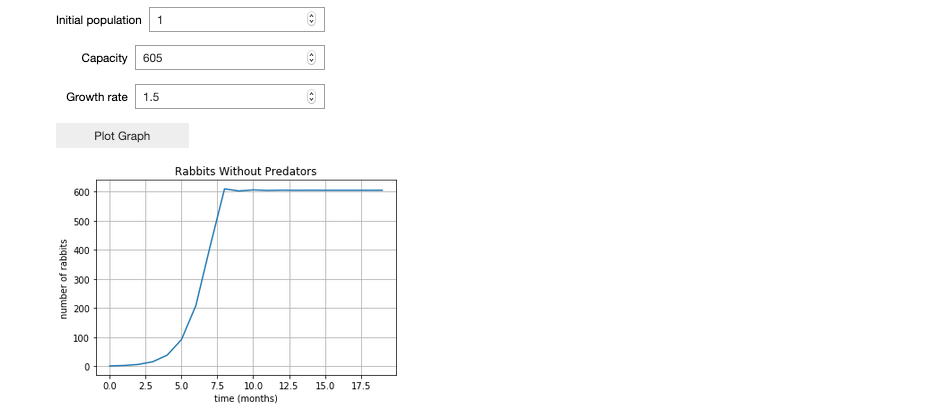
\includegraphics[width = \linewidth, frame]{Figures/1}}
			\caption{Interaction for different initial rabbit population, growth rate and population capacity }
		\end{figure}
		
		One important interaction is the growth rate, as we change from 1.5 to 3, the population dynamics of the rabbits become no longer stable.
			\begin{figure}[H]
			\frame{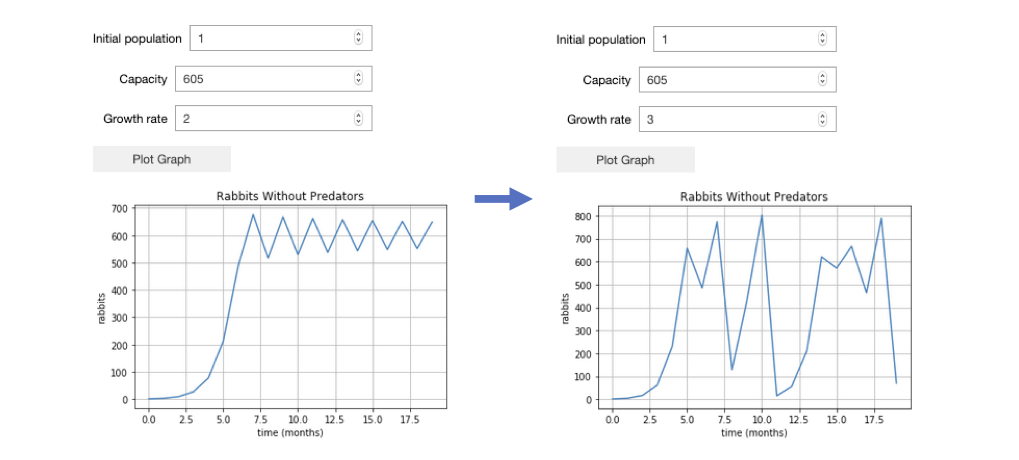
\includegraphics[width = \linewidth, frame]{Figures/t1}}
			\caption{Changing of growth rate lead to unstable population }
		\end{figure}
		
		We could review our growth rate formula of the rabbit by changing the original formula. In current formula, there is a shaping factor. This shaping factor could be generalized to situation such as mass destruction due to destruction of fores, or more natural condition such as different in food source for different seasons.
		
		\begin{figure}[H]
			\frame{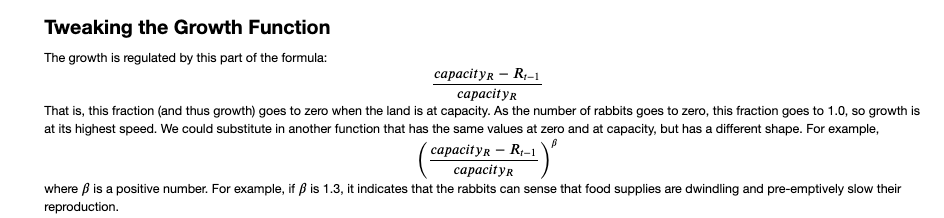
\includegraphics[width = \linewidth, frame]{Figures/1_4}}
			\caption{Changing of growth formula }
		\end{figure}
	
		With such changes, now we have more simulate that rabbit could sense how much the food supplies are dwinding by changing their reproductive condition. With such interaction, even with the same growth rate of 3. Once we throttled their overall growth rate by this shaping condition, we could get a more realistic population dynamic.
			\begin{figure}[H]
			\frame{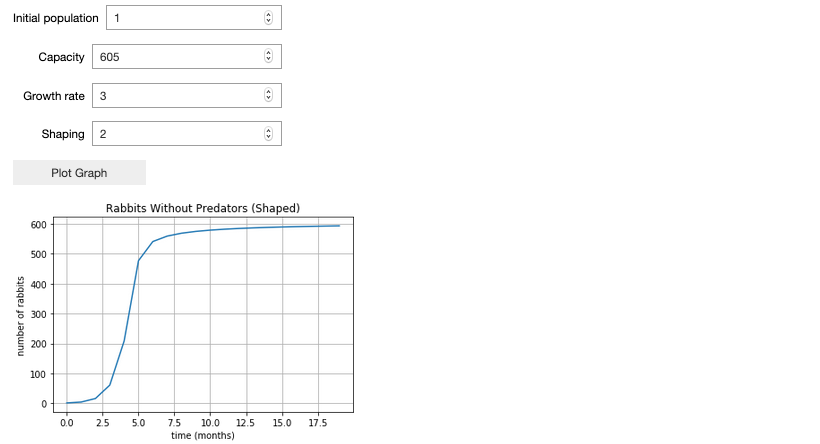
\includegraphics[width = \linewidth, frame]{Figures/1_5}}
			\caption{With shaping force, the rabbit population become stable}
		\end{figure}
		
		\subsubsection{Part 2: Coyote without preys}
		In part 2, we introduce basic predator (coyotes) without preys. It is obvious that the formula will be a decreasing function. Since without preys, coyotes will die due to lack of food source.
			\begin{figure}[H]
			\frame{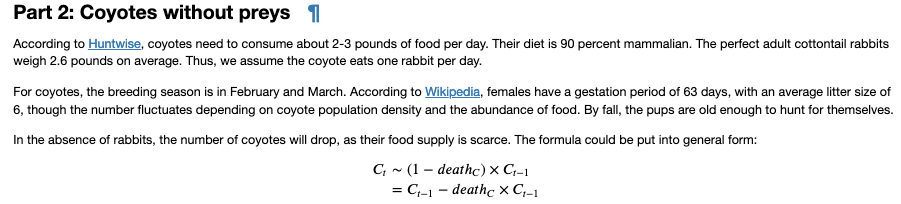
\includegraphics[width = \linewidth, frame]{Figures/2}}
			\caption{Introduce coyote population without preys formula}
				\end{figure}
		We allows users to change how fast coyotes die, as well as their initial population.
			\begin{figure}[H]
			\frame{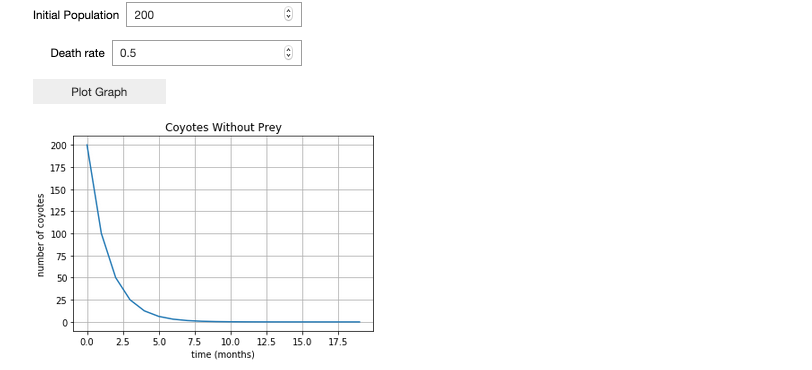
\includegraphics[width = \linewidth, frame]{Figures/3}}
			\caption{Interaction for different initial coyote pupulation and dead rate}
		\end{figure}
	
	\subsubsection{Part 3: Interaction between coyotes and rabbits}
	In part 3, we start to allow interaction between coyotes and rabbits.
			\begin{figure}[H]
			\frame{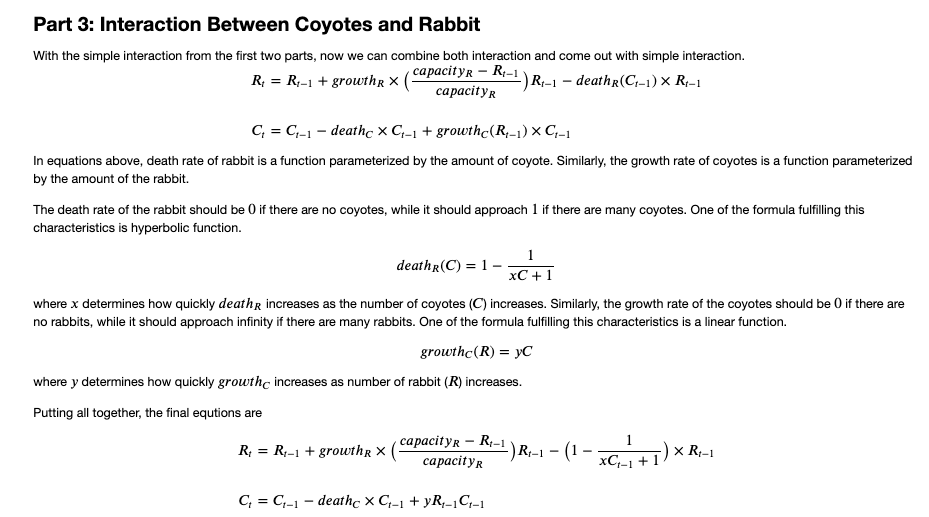
\includegraphics[width = \linewidth, frame]{Figures/4}}
			\caption{Interaction between coyotes and rabbits}
		\end{figure}
	Users have control for rabbit and coyote initial population, capacity for the rabbit, growth rate for rabbit and death rate for coyote. From the formula, we know the x and y are two new parameters introduced in current interactions. Specifically, x  determine how quickly rabbits are decreasing when the coyotes increases; whereas y decides how quickly coyotes are increasing when more rabbits are available.
	\begin{figure}[H]
		\frame{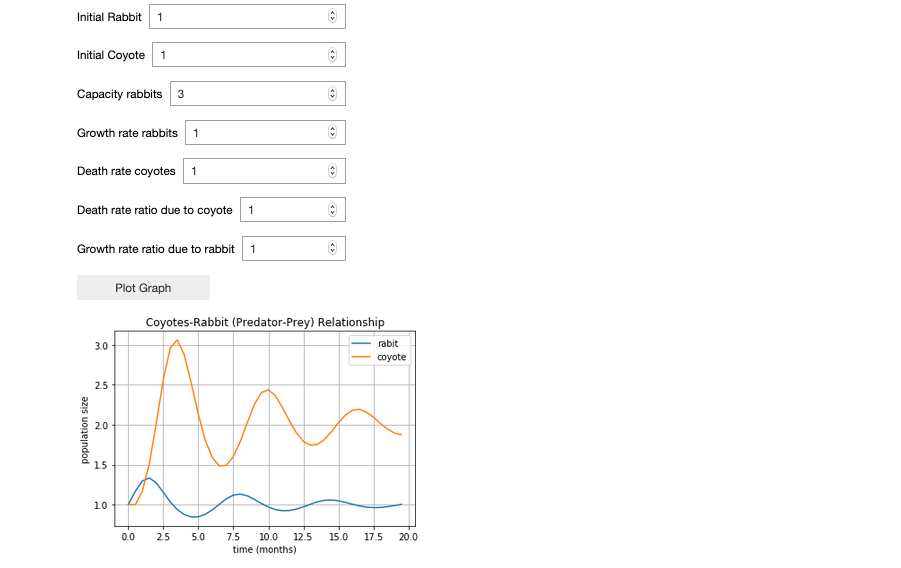
\includegraphics[width = \linewidth, frame]{Figures/5}}
		\caption{Users able to control interaction between coyotes and rabbits}
	\end{figure}
	In our model, it is obvious that the capacity of the rabbit decides the most of the population dynamic, since the coyotes are always hungry and always want to eat and reproduce in this case. 
	
		\subsubsection{Part 4: Trajectories and Direction Fields for a system of equations}
		By looking at the trajectories and direction fields of a system of the predator and prey population, we could gain insight about their relationship.
		\begin{figure}[H]
		\frame{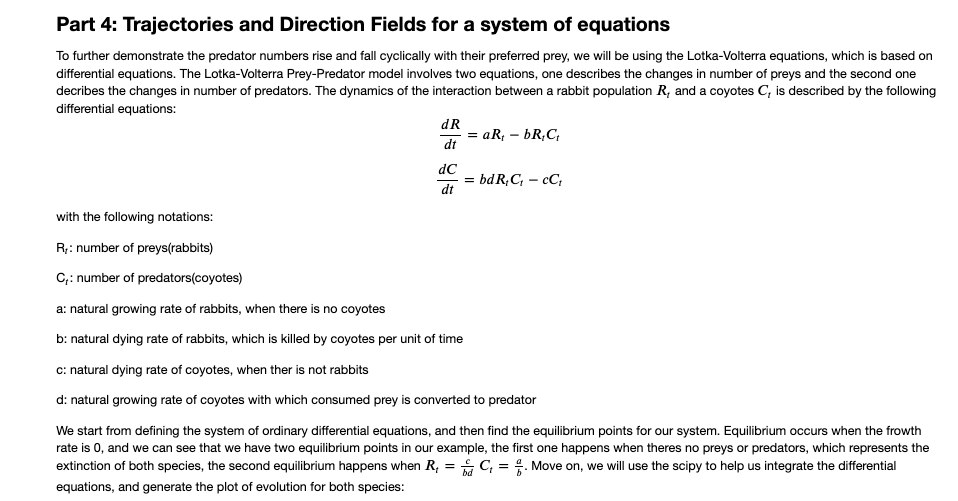
\includegraphics[width = \linewidth, frame]{Figures/p4}}
		\caption{Introduce trajectories and direction fields for interaction between coyotes and rabbits}
		\end{figure}
	We allows users to tune the a, b, c and d parameters to see the interaction. 
		\begin{figure}[H]
		\frame{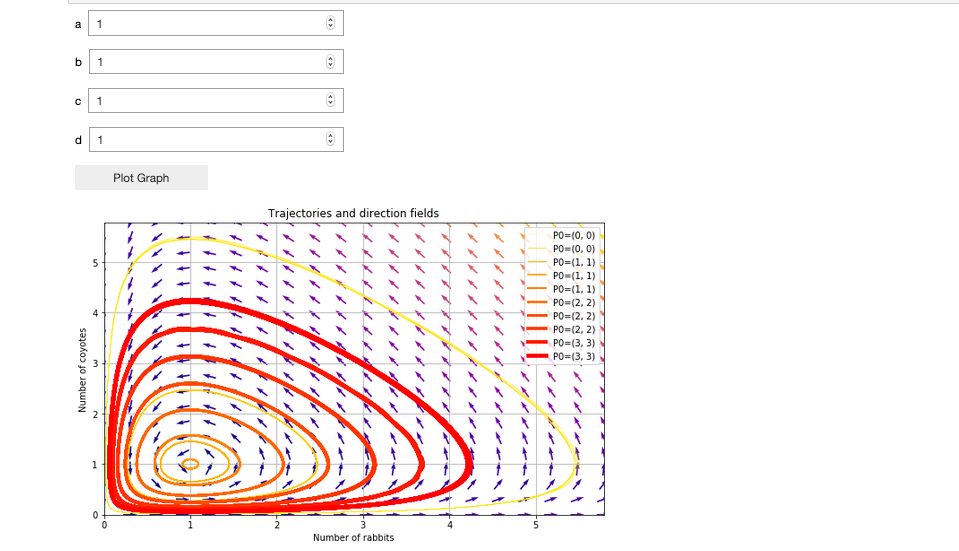
\includegraphics[width = \linewidth, frame]{Figures/p4-1}}
		\caption{Trajectories and direction fields for interaction between coyotes and rabbits}
		\end{figure}	
	\subsubsection{Part 5: Multiple predators and preys relationship}
	We could extends our current model to multiple predators and preys relationship. The relationship is similar to the one predator one prey relationship. We assume each preys will give the same growth rate to the predators, while the predators will cause same death rate to the preys. While we could change such relationship to one to one condition, such changes may not further improve our understanding on the relationship. We could assume our case as special case where the growth rate are the same.
		We allows users to tune the different initial population, growth rate and death rate of different species to see the interaction. 
	\begin{figure}[H]
		\frame{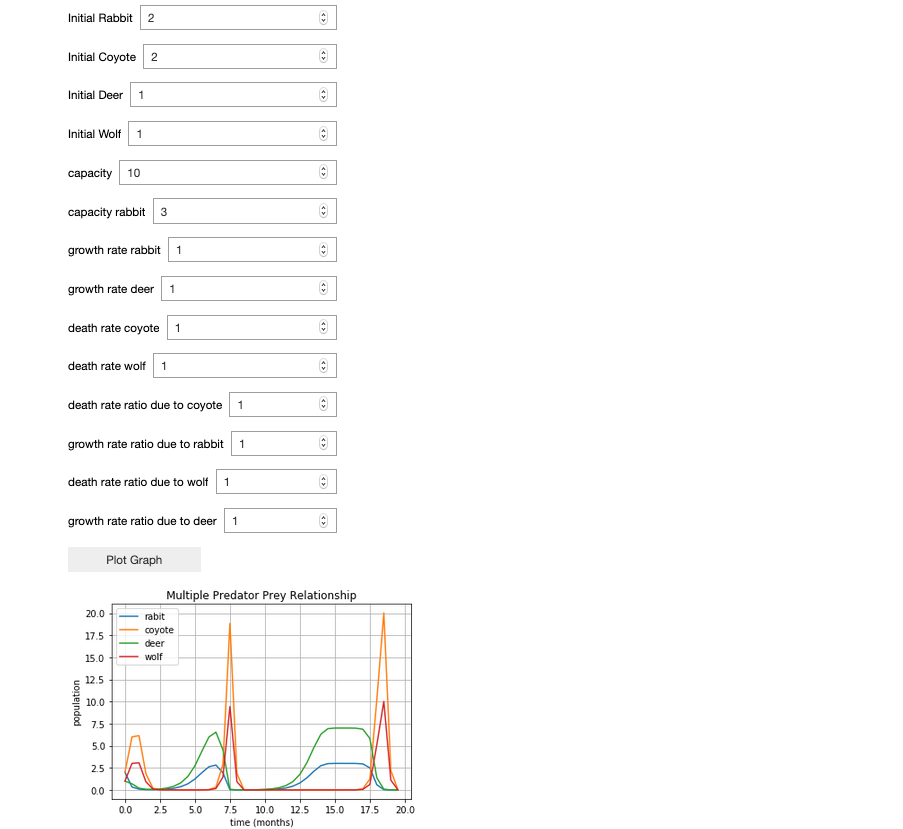
\includegraphics[width = \linewidth, frame]{Figures/final}}
		\caption{Interaction between multiple predators (wolves and coyotes) and preys (rabbits and deers)}
	\end{figure}

\newpage
\subsection{Cellular Automata}
\subsubsection{Introduction to the world}
\begin{figure}[H]
	\frame{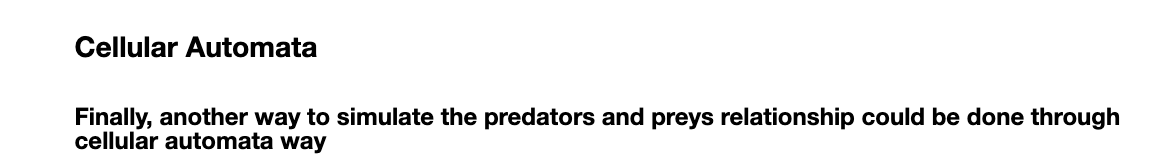
\includegraphics[width = \linewidth, frame]{Figures/c1}}
	\caption{Introduction to Cellular Automata}
\end{figure}
Some information will be introduced:
\begin{enumerate}
	\item Possible states : EMPTY = 0; PREY = 1; PREDATOR = 2.
	\item The world was created using 2D numpy array. 
\end{enumerate}
\begin{figure}[H]
	\frame{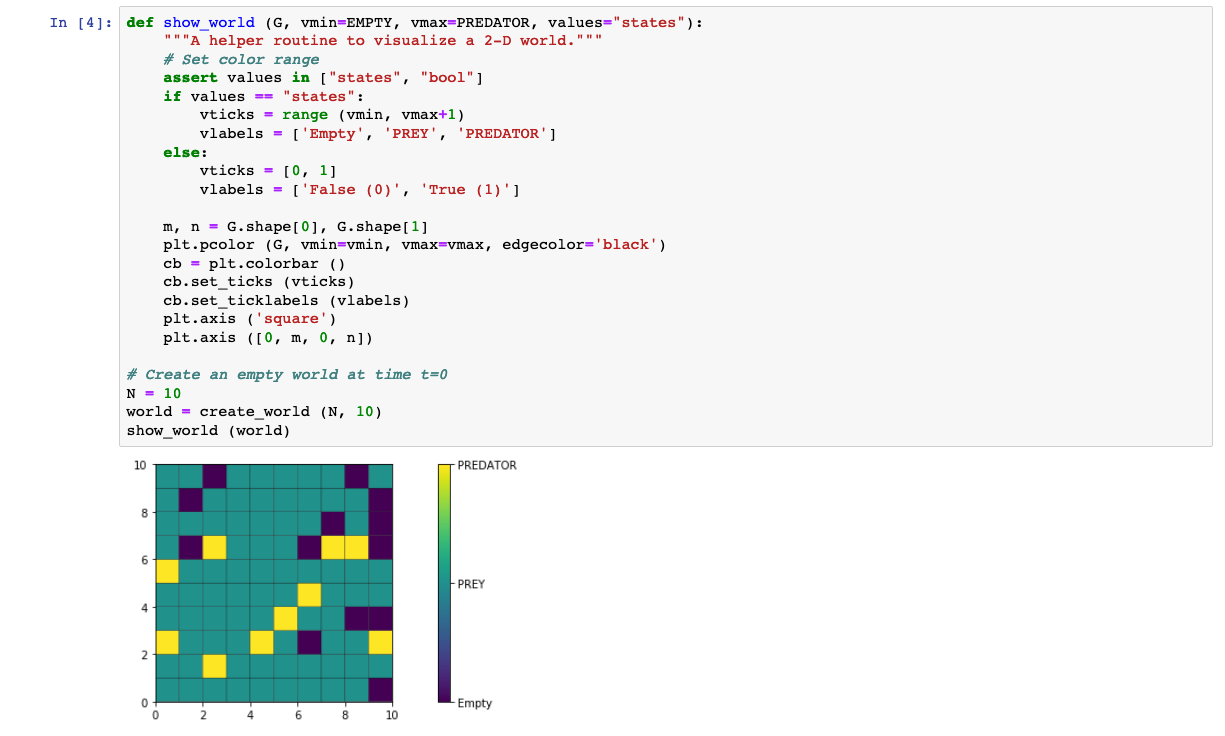
\includegraphics[width = \linewidth, frame]{Figures/c3}}
	\caption{Introduction to Cellular Automata World}
\end{figure}
\subsubsection{Utility functions}
We requires users to create several functions: This to identify the empty space, prey and predator in the world.
\begin{figure}[H]
	\frame{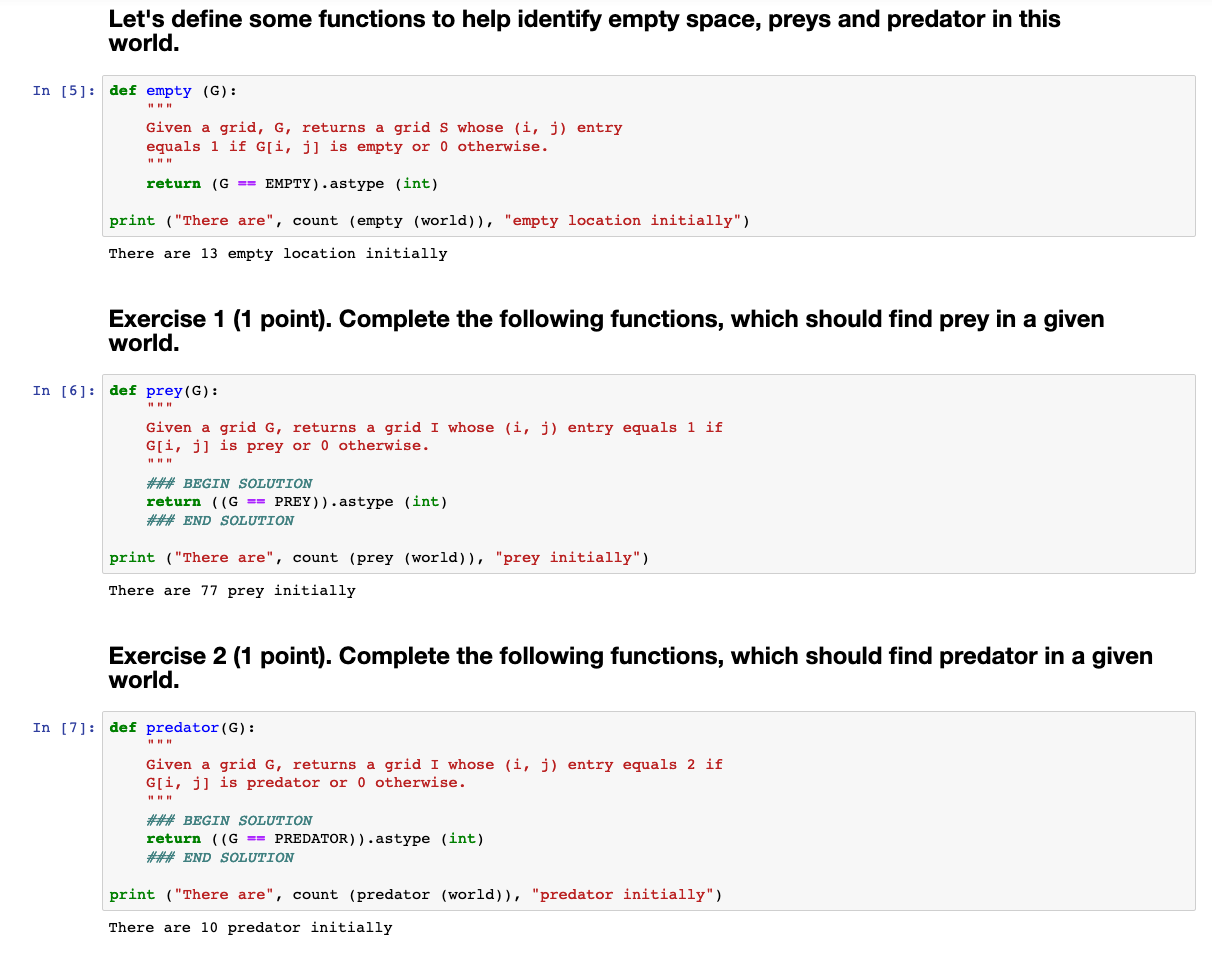
\includegraphics[width = \linewidth, frame]{Figures/c4}}
	\caption{Some utility functions}
\end{figure}
\subsubsection{Get\_neighbor functions}
Get neighbor function is important since cellular automata has space relationship among preys and predators. Predators can only eat preys within thier neigborhood. Both prey and predators can only move to their neighborhood.
\begin{figure}[H]
	\frame{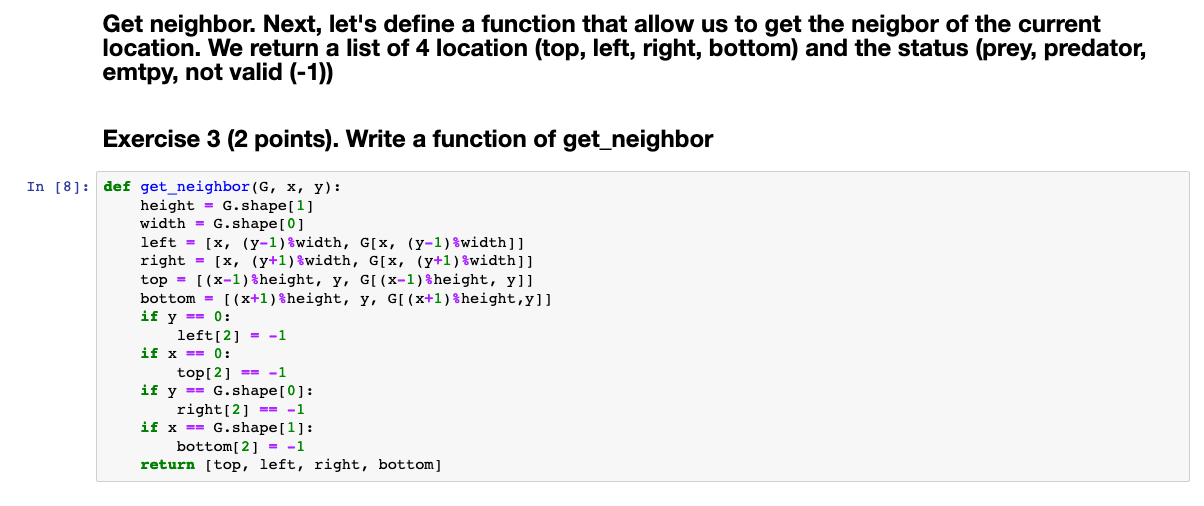
\includegraphics[width = \linewidth, frame]{Figures/c5}}
	\caption{Get neighbor functions}
\end{figure}

\subsubsection{Predator movement functions}
Once we have the get\_neighbor function, we could write the movement function. We start with movement of predators. We list the assumptions.
\begin{enumerate}
	\item If any of the neighbor is prey, predator will randomly move to that location and eat the prey, or has offspring occupy that space according to reproductive probability.
	\item If the location is empty, it will move to that location randomly.
	\item Without food, it may die according to the dying probability.
\end{enumerate}
\begin{figure}[H]
	\frame{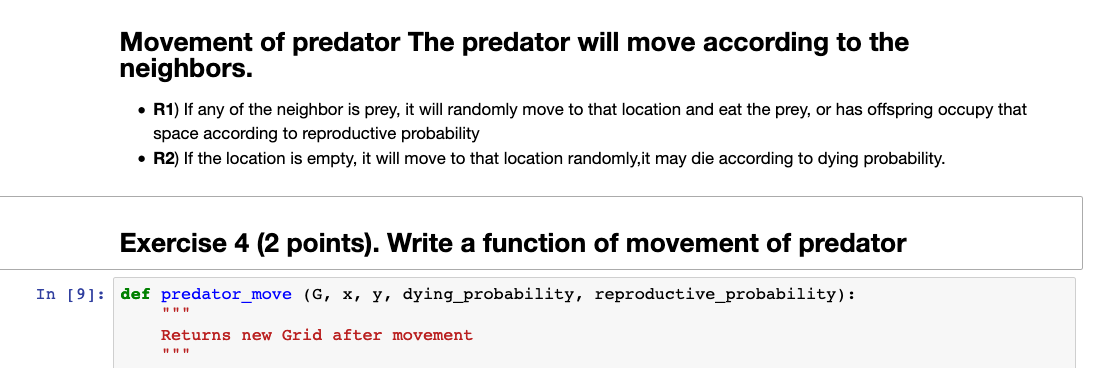
\includegraphics[width = \linewidth, frame]{Figures/c6}}
	\caption{Predator movement function}
\end{figure}

\subsubsection{Prey movement functions}
Similarly, we need to write the prey movement. The condition is much easier, if there is any empty space, prey could move to the location, or they can have their offspring there according to the reproductive probability.
\begin{figure}[H]
	\frame{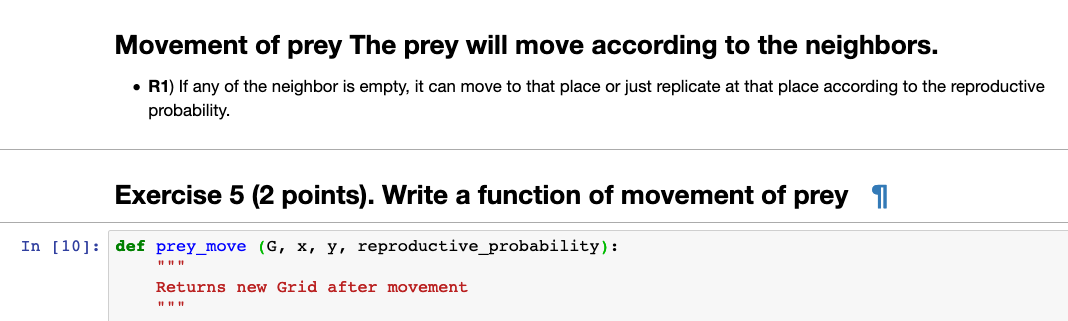
\includegraphics[width = \linewidth, frame]{Figures/c8}}
	\caption{Prey movement function}
\end{figure}

\subsubsection{Step functions}
We provide step function for each step of the simulation. 
\begin{figure}[H]
	\frame{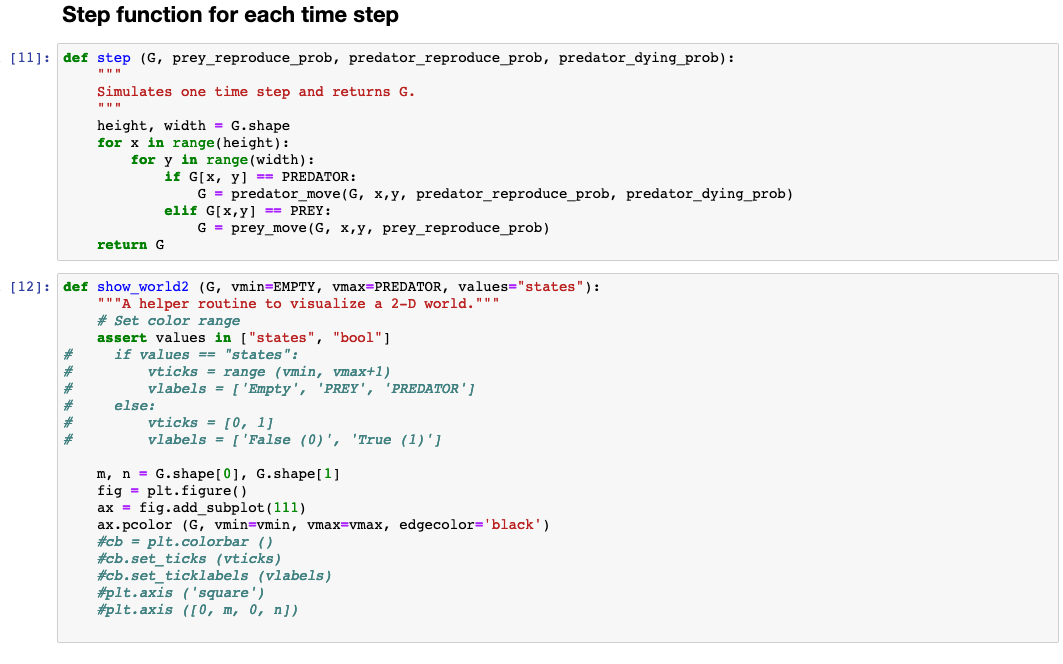
\includegraphics[width = \linewidth,frame]{Figures/c9}}
	\caption{Step function}
\end{figure}

\subsubsection{Putting alltogether}
Finally, we put all the functions written together. 
\begin{figure}[H]
	\frame{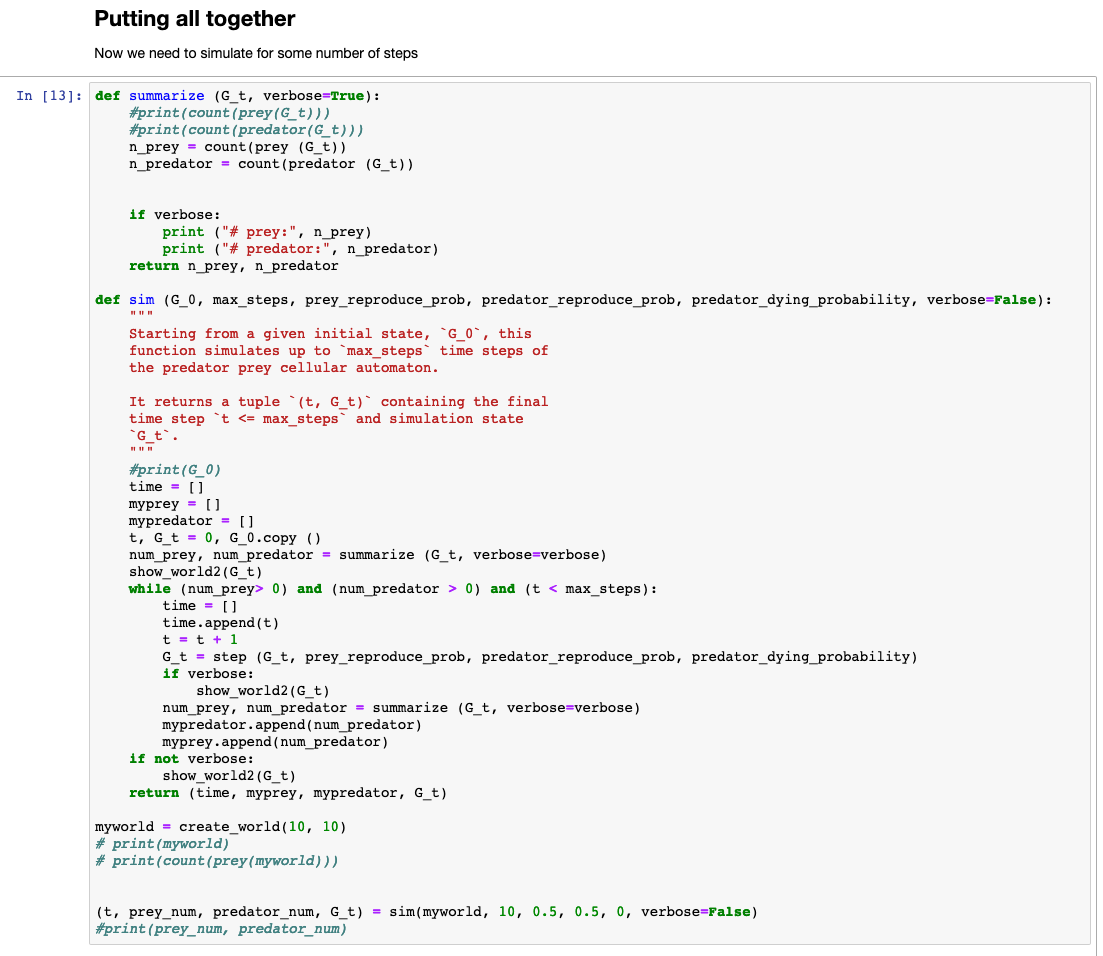
\includegraphics [width = \linewidth, frame]{Figures/c11}}
	\caption{Putting all functions together}
\end{figure}
We also provide a interactive user input and button for users to try different value.
\begin{figure}[H]
	\frame{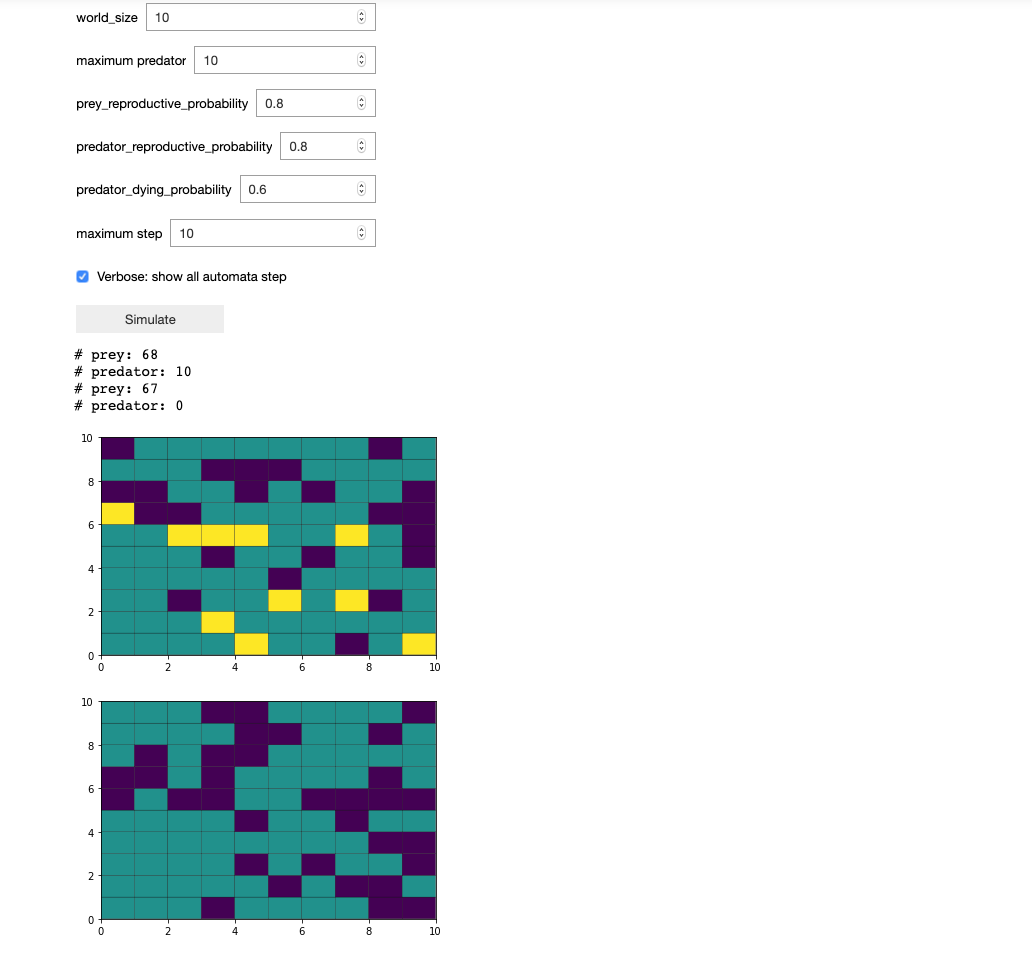
\includegraphics[width = \linewidth,frame]{Figures/c12}}
	\caption{Users interaction}
\end{figure}
\newpage
\subsection{Agent Based Simulation / Agent Based Model}
\subsubsection{Introduction to the Agent-Based Simulation model framework}
\begin{figure}[H]
	\frame{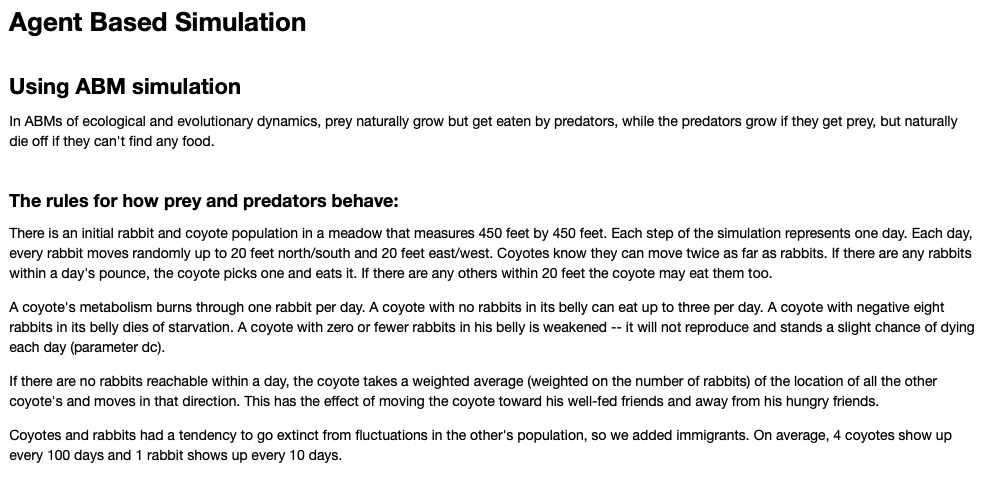
\includegraphics[width = \linewidth, frame]{Figures/abs1}}
	\caption{Introduction to ABS framework}
\end{figure}
\subsubsection{Embedded version}
We have one embedded version that could support step function. The red spot is the predator (coyote), while the black spot is the rabbit (preys). Users press init, then step through the simulation.
\begin{figure}[H]
	\frame{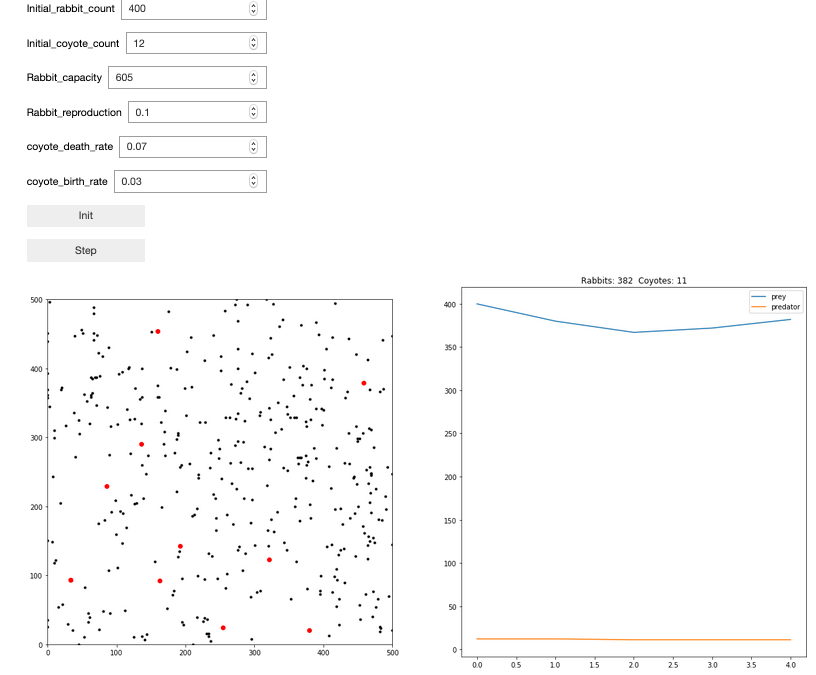
\includegraphics[width = \linewidth,frame]{Figures/static_abs}}
	\caption{Embedded version}
	\end{figure}
\subsubsection{GUI version}
We used GUI framework available from Sayama.et al \cite{Sayama2013} to develop our model.
At Jupyter Notebook, when running the simulation, we will have a working GUI. The red spot is the predator (coyote), while the black spot is the rabbit (preys).
\begin{figure}[H]
	\frame{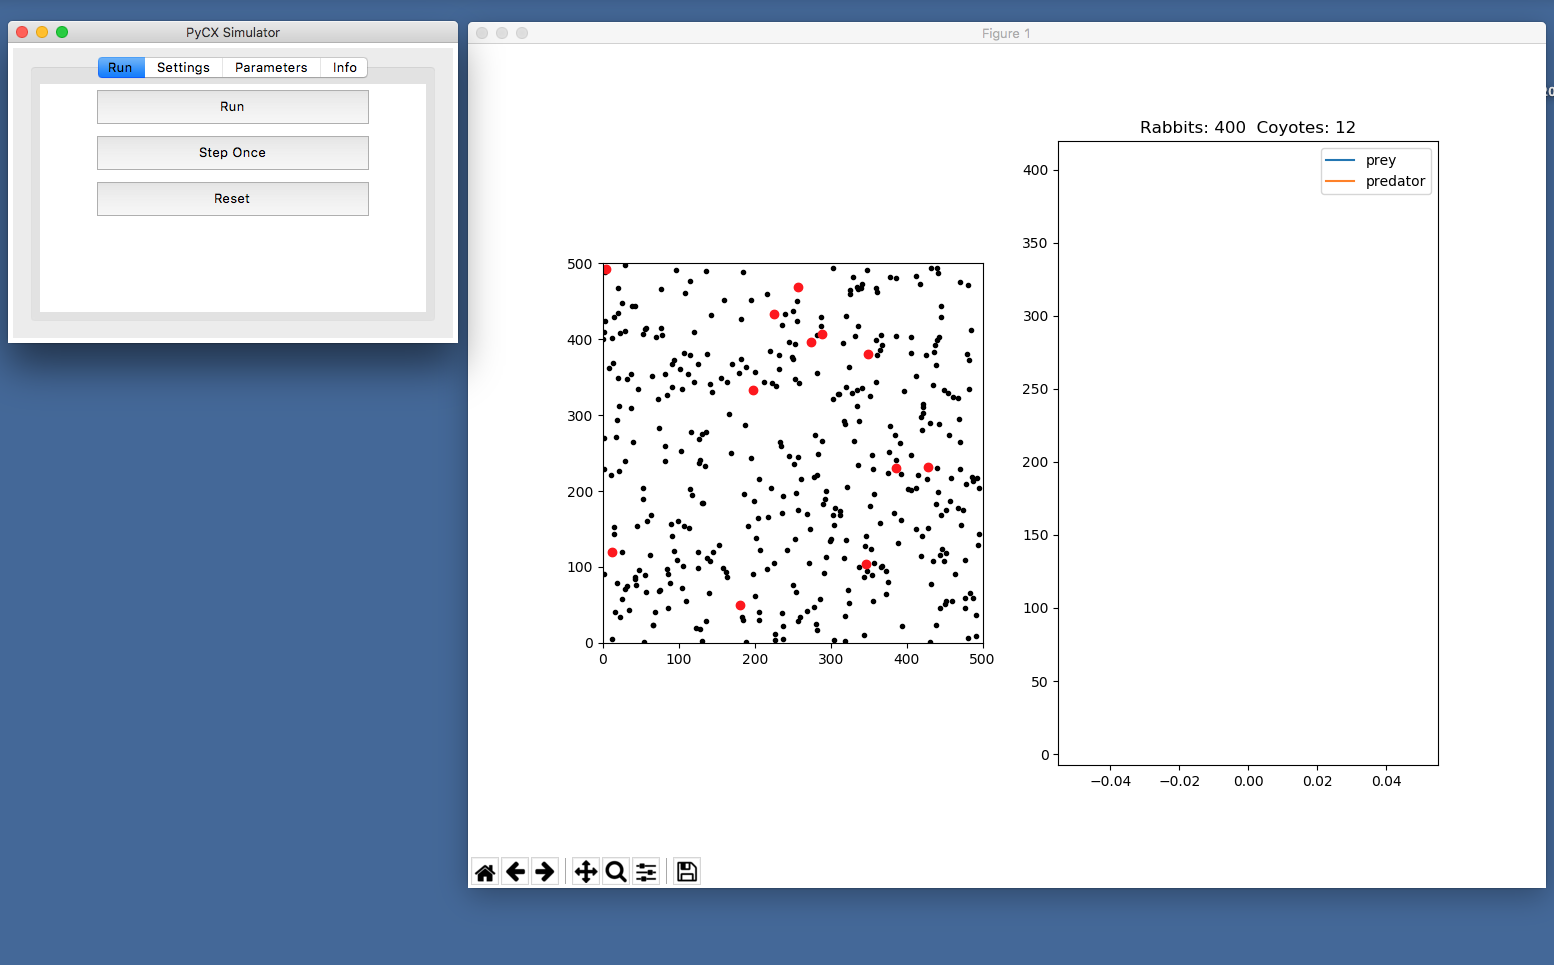
\includegraphics[width = \linewidth,frame]{Figures/ABS_Start}}
	\caption{Start of ABS Simulation}
\end{figure}

\newpage
\subsubsection{Continuous run of simulation}
Pressing run will enable the simulation to occurs, presssing pause will hold the simulation. The begining of the predators and preys are randomly initialized.
\begin{figure}[H]
	\frame{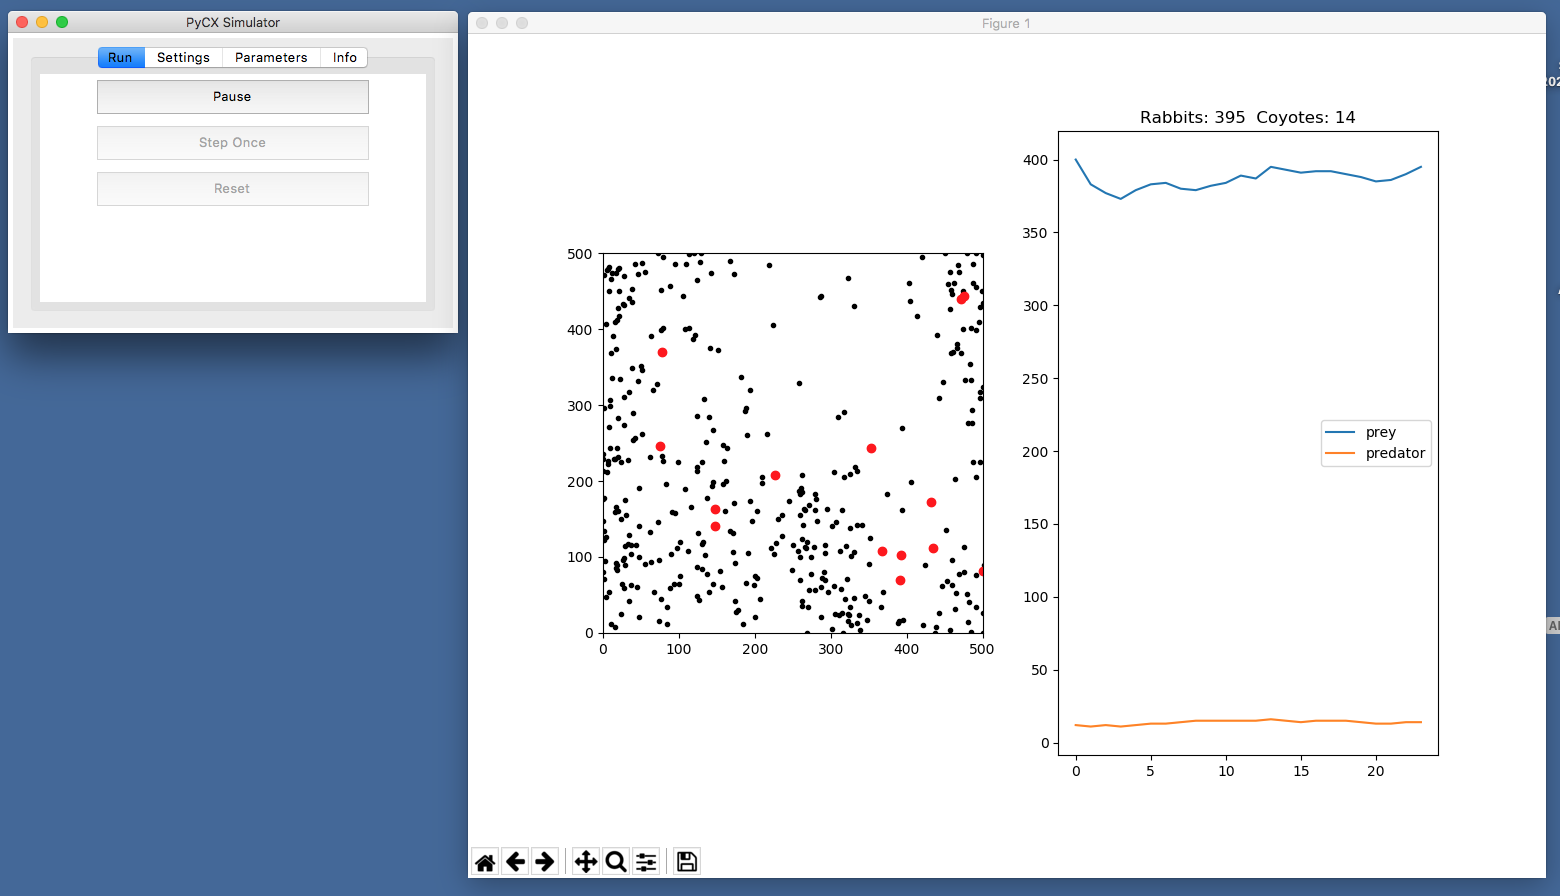
\includegraphics[width = \linewidth, frame]{Figures/ABS_run}}
	\caption{Running of ABS Simulation}
\end{figure}
\begin{figure}[H]
	\frame{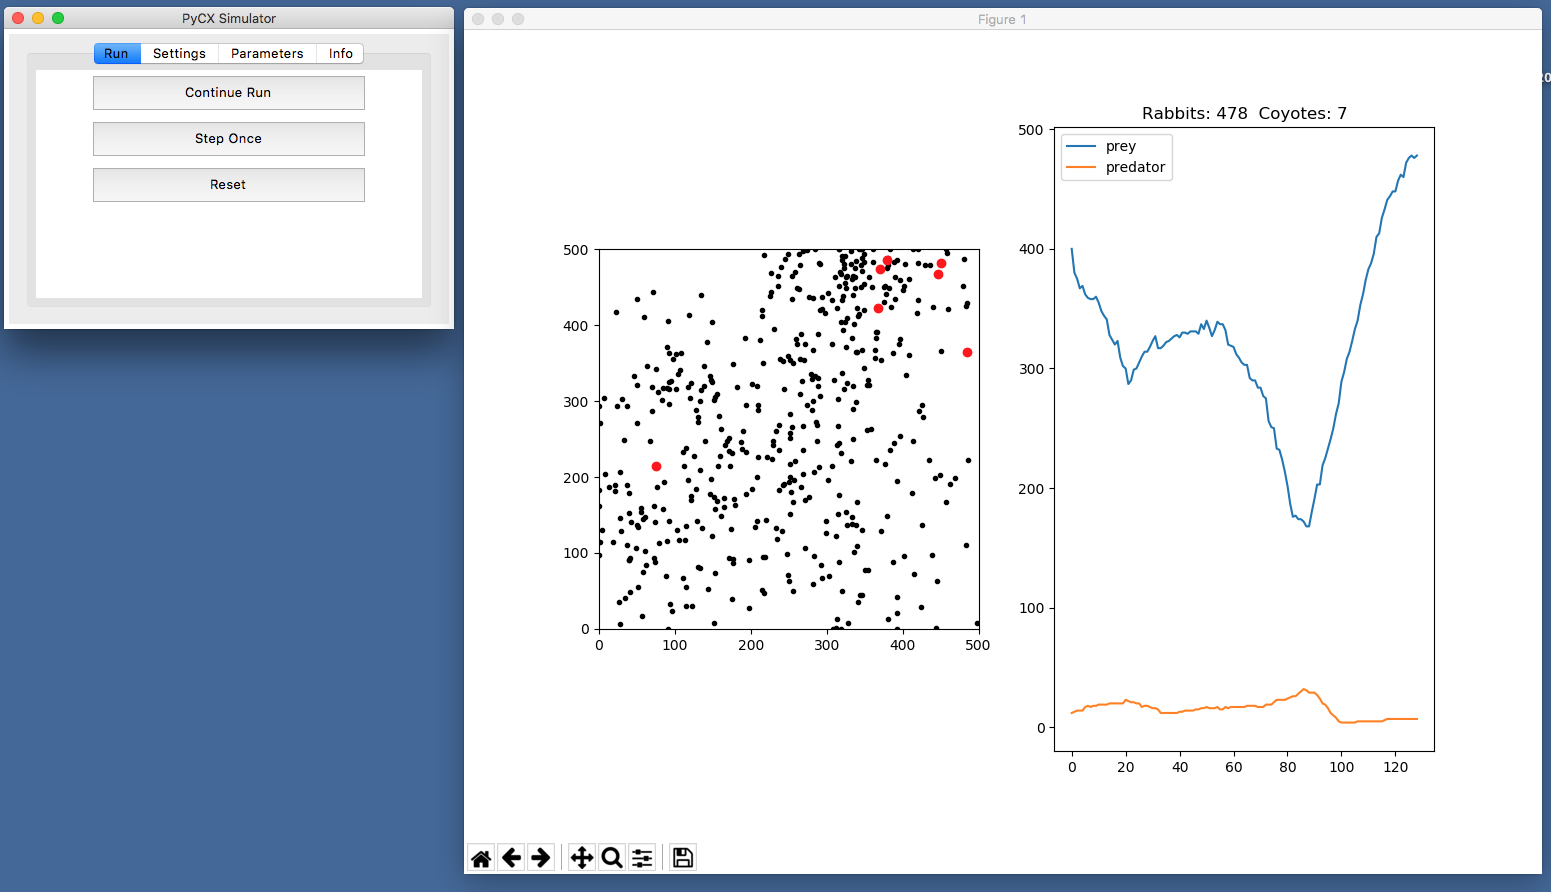
\includegraphics[width = \linewidth,frame]{Figures/ABS_run_pause}}
	\caption{Pause of ABS Simulation}
	\end{figure}

\newpage
\subsubsection{Stepping of simulation}
Users can also choose to step through the simulation. We show randomly two screen shots after different steps for the simulation.
\begin{figure}[H]
	\frame{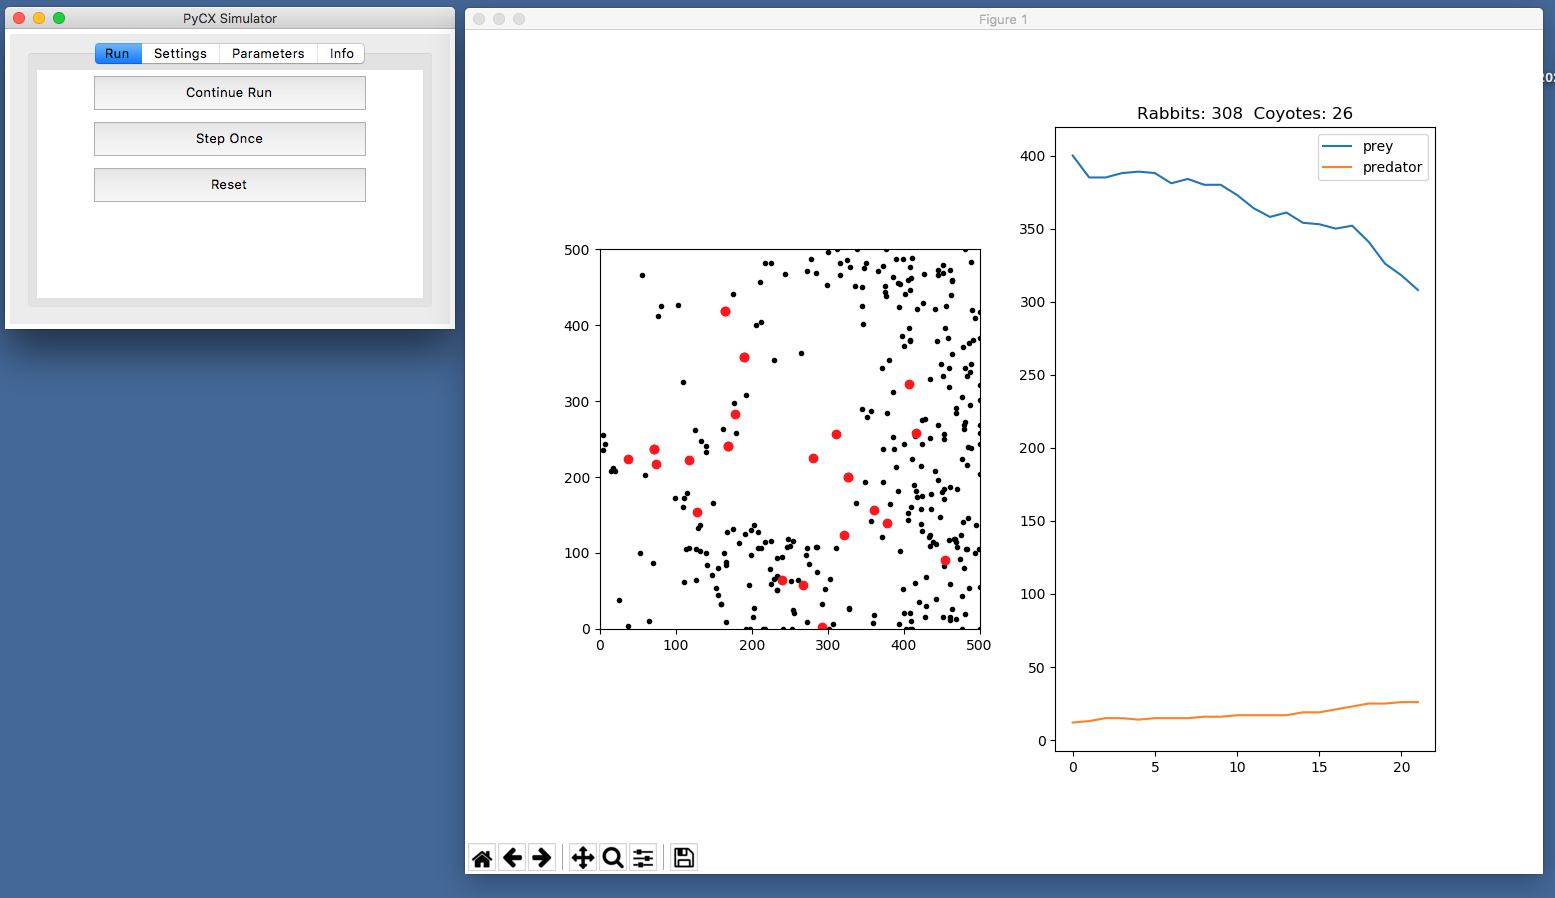
\includegraphics[width = \linewidth,frame]{Figures/ABS_step}}
	\caption{Stepping of Simulation 1}
\end{figure}

\begin{figure}[H]
	\frame{\includegraphics[width = \linewidth,frame]{Figures/ABS_25step}}
	\caption{Stepping of Simulation 2}
\end{figure}

\newpage
\subsubsection{Parameters setup}
Users are allowed to control the initial rabbit population, coyote population, rabbit capacity, rabbit reproduction, coyote death rate and birth rate in the Parameters tab.
\begin{figure}[H]
	\frame{\includegraphics[scale=0.5]{Figures/ABS_Parameters}}
	\caption{Parameters setup}
\end{figure}

\subsubsection{Simulation settings}
Users are allows to change some of the simulation settings, such as step side and how fast the visualization delay.
\begin{figure}[H]
	\frame{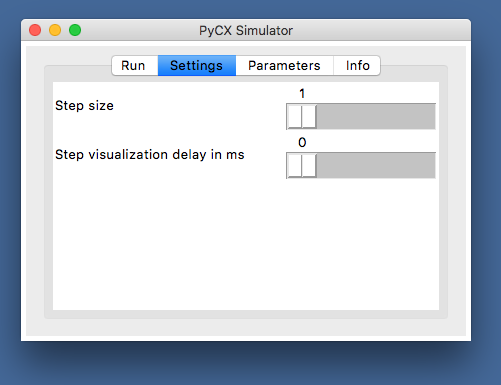
\includegraphics[scale=0.5]{Figures/ABS_settings}}
	\caption{Simulation settings}
\end{figure}

\subsubsection{Information}
Finally, some additional information.
\begin{figure}[H]
	\frame{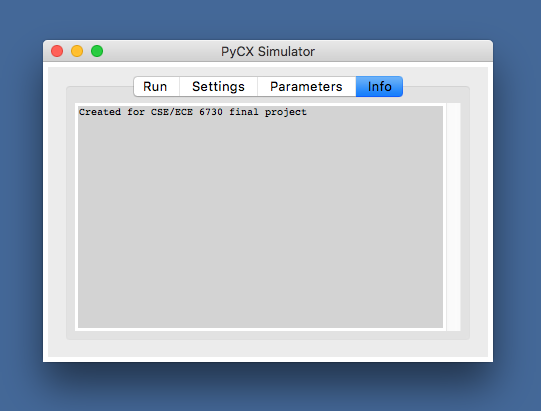
\includegraphics[scale=0.5]{Figures/Info}}
	\caption{Additional Information}
\end{figure}

\subsection{Event-based Simulation}

\subsubsection{Introduction}

\begin{figure}[H]
	\frame{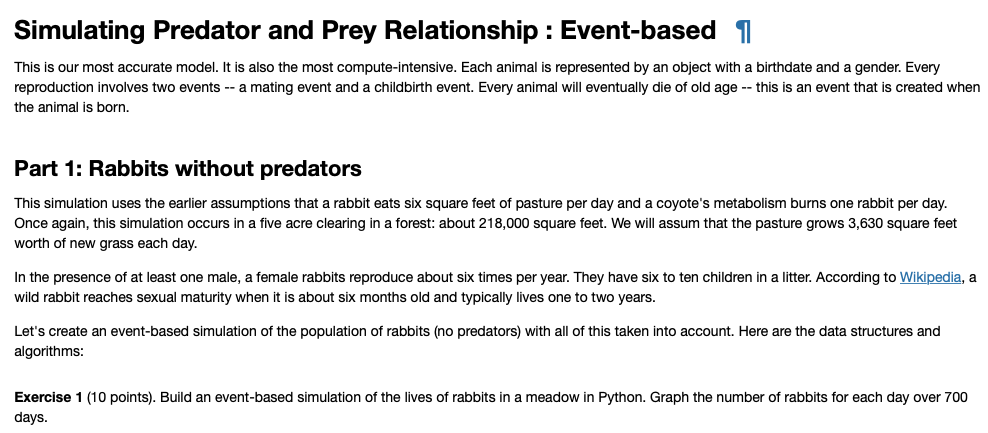
\includegraphics[width = \linewidth,frame]{Figures/eventintro.png}}
	\caption{Introduction to Event-Based Simulation}
\end{figure}

\subsubsection{Just Rabbits}

\begin{figure}[H]
	\frame{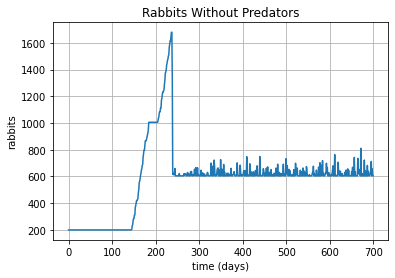
\includegraphics[scale=0.6,frame]{Figures/eventrabbit.png}}
	\caption{Rabbits only}
\end{figure}

This is what the simulation does for just rabbits.  Note that in this simulation, which is our most accurate, there is a dramatic die-off.  It seems that rabbits are reproducing at their fastest rate just as the meadow becomes over grazed.  The system then settles near equilibrium very quickly.

\subsubsection{Add Coyotes}

\begin{figure}[H]
	\frame{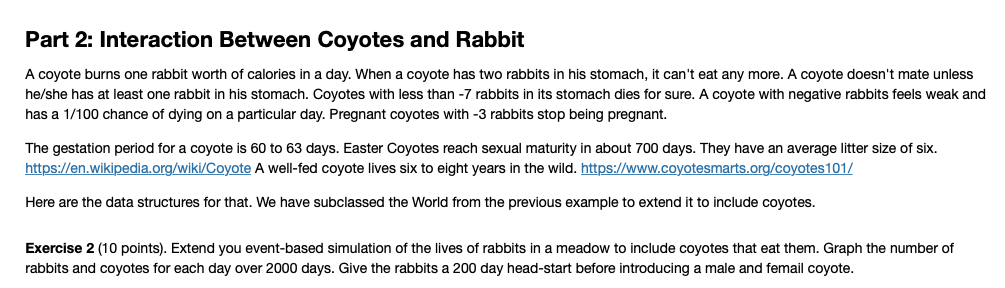
\includegraphics[width = \linewidth,frame]{Figures/eventintrocoyote.png}}
	\caption{Adding Coyotes}
\end{figure}

We give the rabbits a 200 day headstart to get to equilibrium with their meadow before introducing two coyotes.

\begin{figure}[H]
	\frame{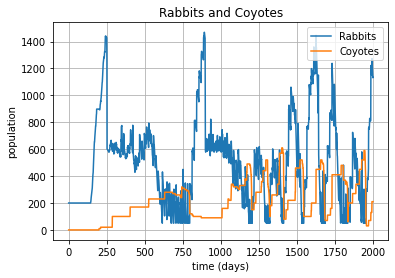
\includegraphics[scale=0.6,frame]{Figures/eventrabbitcoyote.png}}
	\caption{Coyotes and Rabbits}
\end{figure}





		\section{Division of Labor}
		As we move forward on our project, we plan to work concurrently. The timeline is as below:
		
		\begin{center}
			\begin{tabular}{ |c|c|c| } 
				\hline
				Task & Duration  \\ 
				\hline
				Literature review & 2 weeks \\ 
				Modeling design and implementaion & 4 weeks \\ 
				Modeling revised & 4 weeks \\ 
				\hline
			\end{tabular}
		\end{center}
	
		\begin{center}
			\begin{tabular}{ |c|c|c| } 
				\hline
				Task & Member  \\ 
				\hline
				Literature review & All members\\			
				Event-based Simulation & D. Aaron Hillegass\\ 
				Single predator model, trajectories and direction field & Xiaotong Mu\\
				UI interaction, predator prey interaction (single and multiple) & Siawpeng Er\\
				Agent Based Simulation & All members\\
				Cellular Automata & All members\\
				Event Based Simulation & All members\\
				Final Report & All members \\
				\hline
			\end{tabular}
		\end{center}

		
		\bibliographystyle{plain}
		\bibliography{reference}
	\end{normalsize}
	
\end{document}
